\documentclass{beamer}

\usepackage{helvet}
\usepackage{hyperref, graphicx}
\usepackage{amsthm}
\usepackage{etoolbox}
\usepackage{multicol}

\usetheme[progressbar=frametitle, numbering=none]{metropolis}
\usecolortheme[snowy]{owl}
\setbeamertemplate{navigation symbols}{}
\AtBeginSection[ ]
{
\begin{frame}{Outline}
    \tableofcontents[currentsection]
\end{frame}
}

% Default fixed font does not support bold face
\DeclareFixedFont{\ttb}{T1}{txtt}{bx}{n}{11} % for bold
\DeclareFixedFont{\ttm}{T1}{txtt}{m}{n}{12}  % for normal - use in headings

% Custom colors
\usepackage{color}
\definecolor{TUGray}{RGB}{101,101,137}
\definecolor{TUBlack}{RGB}{0,0,10}
\definecolor{mygreen}{RGB}{45,111,63}
\definecolor{keywords}{RGB}{205,114,0}
\definecolor{comments}{RGB}{181,51,139}
\definecolor{strings}{RGB}{58,144,81}
\definecolor{numeric}{RGB}{66,110,176}
\definecolor{linos}{rgb}{0.4,0.4,0.4}
\definecolor{links}{rgb}{0,0.4,0.75}

\definecolor{bggray}{RGB}{232, 233, 235}

\setbeamercolor{alerted text}{fg=mygreen}
\setbeamercolor{normal text}{fg=TUBlack}\usebeamercolor*{normal text}

\setbeamercolor{codecol}{fg=TUGray!25!black,bg=bggray}

\hypersetup{colorlinks, linkcolor=links, urlcolor=links}

\usepackage[T1]{fontenc}
\usepackage[sfdefault,scaled=.85]{FiraSans}
\usepackage{newtxsf}

\usepackage{listings}

\newtoggle{InString}{}% Keep track of if we are within a string
\togglefalse{InString}% Assume not initally in string

\newcommand\digitstyle{\color{numeric}}
\makeatletter
\newcommand{\ProcessDigit}[1]
{%
  \ifnum\lst@mode=\lst@Pmode\relax%
   {\digitstyle #1}%
  \else
    #1%
  \fi
}
\makeatother

\lstset{literate=%
    {0}{{{\ProcessDigit{0}}}}1
    {1}{{{\ProcessDigit{1}}}}1
    {2}{{{\ProcessDigit{2}}}}1
    {3}{{{\ProcessDigit{3}}}}1
    {4}{{{\ProcessDigit{4}}}}1
    {5}{{{\ProcessDigit{5}}}}1
    {6}{{{\ProcessDigit{6}}}}1
    {7}{{{\ProcessDigit{7}}}}1
    {8}{{{\ProcessDigit{8}}}}1
    {9}{{{\ProcessDigit{9}}}}1
	{<=}{{\(\leq\)}}1
	{>=}{{\(\geq\)}}1,
	% morestring=[b]",
    % morestring=[b]',
    % morecomment=[l]{//},
}

\lstdefinelanguage{Pseudo}{
    morekeywords={begin, end, return, while},
    morecomment=[l]{\#},
}

% Pseudocode style
\newcommand\pseudostyle{\lstset{
language=Pseudo,
basicstyle=\fontfamily{ccr}\scriptsize,
commentstyle=\it\scriptsize\color{linos},
keywordstyle=\it\bfseries\scriptsize,
mathescape=true,
literate=
    {=}{$\leftarrow{}$}{1}
    {==}{$={}$}{1},
xleftmargin=18pt,
xrightmargin=4pt,
aboveskip=12pt,
belowskip=0pt,
frame=tB,
keepspaces=true
}}

% Python style for highlighting
\newcommand\pythonstyle{\lstset{
language=Python,
basicstyle=\ttfamily\tiny,
numbers=left,
numberstyle=\tiny\color{linos},
morekeywords={self, np},              % Add keywords here
keywordstyle=\tiny\color{keywords},
commentstyle=\it\tiny\color{comments},    % Custom highlighting style
stringstyle=\tiny\color{strings},
xleftmargin=18pt,
xrightmargin=4pt,
aboveskip=0pt,
belowskip=0pt,
escapeinside={(*@}{@*)},
frame=l,                         % Any extra options here
showstringspaces=false,
keepspaces=true
}}

% Pseudocode environment
\lstnewenvironment{pseudo}[1][]
{
    \pseudostyle
    \lstset{
        #1
    }
}
{}

% Python environment 
\lstnewenvironment{python}[1][]
{
	\pythonstyle
	\lstset{
	#1
	}
}
{}

% wrap the Python environment
\newenvironment{codeblock}
    {\hfill\begin{beamerboxesrounded}[lower=codecol, width=0.8\textwidth]
    \medskip

    }
    { 
    \end{beamerboxesrounded}\hfill
    }

\theoremstyle{example}
\newtheorem{question}{Question}

\newcommand{\ct}[1]{\lstinline[language=Python,basicstyle=\ttfamily\footnotesize,stringstyle=\small\color{strings}]!#1!}
\newcommand{\ttt}[1]{{\small\texttt{#1}}}
\newcommand{\lsitem}[2]{\ttt{{#1}[}\ct{#2}\ttt{]}}
\newcommand{\bb}[1]{\mathbb{#1}}
\newcommand{\cl}[1]{\mathcal{#1}}
\newcommand{\comment}[1]{}

\author{Chris Cornwell}
\date{September 11, 2025}
\title{Linear regression through Optimization}

\begin{document}

\begin{frame}
\titlepage
\end{frame}

\begin{frame}
\frametitle{Outline}
\tableofcontents
\end{frame}

\section{Measuring the fitness of linear models}

\begin{frame}
    \frametitle{Least Squares loss function}
    On given data $({\bf x}_1, y_1), ({\bf x}_2, y_2), \ldots, ({\bf x}_P, y_P)$, the measure that is commonly used for how well a linear regression model, $f_{b,{\bf w}}({\bf x}) = b + {\bf x}^T{\bf w}$, fits the data is the Least Squares loss (cost) function. 
    \vspace*{-8pt}
    \begin{itemize}
        \item \textit{This is $P$ times the Mean Squared Error.}
    \end{itemize}

    Following notation from textbook, this loss function is 
        \[g(b, {\bf w}) = \sum_{p=1}^P\left(f_{b,{\bf w}}({\bf x}_p) - y_p\right)^2.\]
    
    %\centering 
    % 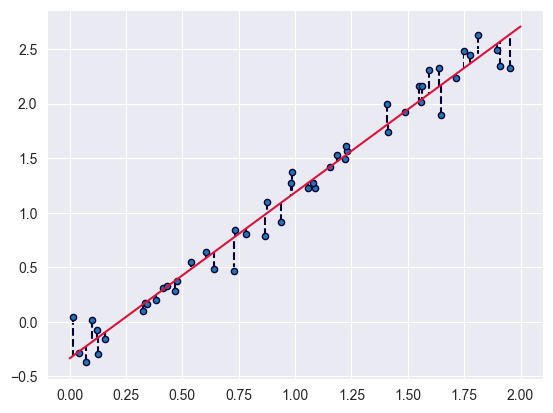
\includegraphics[width=0.4\textwidth]{lsr-error-lines.png}
\end{frame}

\begin{frame}
    \frametitle{Meaning of Least Squares loss}
    For $1\le p\le P$, since $f_{b,{\bf w}}({\bf x}_p) = \hat{y}_p$, the quantity $|f_{b,{\bf w}}({\bf x}_p) - y_p|$ is the vertical distance from $(x_p, y_p)$ to the point predicted by the linear model, $(x_p, \hat{y}_p)$. 

    Additionally, the length of the vector ${\bf y} - \hat{\bf y}$ (which is the distance from ${\bf y}$ to the point determined by $\tilde{\bf w}$, in the column space of our feature matrix) is equal to 
        \[\sqrt{(\hat{y}_1 - y_1)^2 + (\hat{y}_2 - y_2)^2 + \ldots + (\hat{y}_P - y_P)^2} = \sqrt{g(b, {\bf w})}.\]

    We see that minimizing $g(b, {\bf w})$ is the same as minimizing that distance, which will give us the $\hat{\bf y}$ in the column space that makes ${\bf y} - \hat{\bf y}$ be orthogonal to the column space.
\end{frame}

\begin{frame}
    \frametitle{Minimizing the Least Squares loss}
    The data $\{({\bf x}_p, y_p)\}_{p=1}^P$ is fixed. How do we solve the problem 
                \[\underset{\text{minimize}}{b,{\bf w}} g(b, {\bf w})?\]
    We can use methods from calculus, specifically the first order condition {--} that we want all partial derivatives equal to zero. 
    \begin{itemize}
        \item Note, what are the variables of the function $g$?  They are the parameters $b,w_1,w_2,\ldots,w_N$.
    \end{itemize}
\end{frame}

\end{document}